\usetikzlibrary{shapes.geometric}


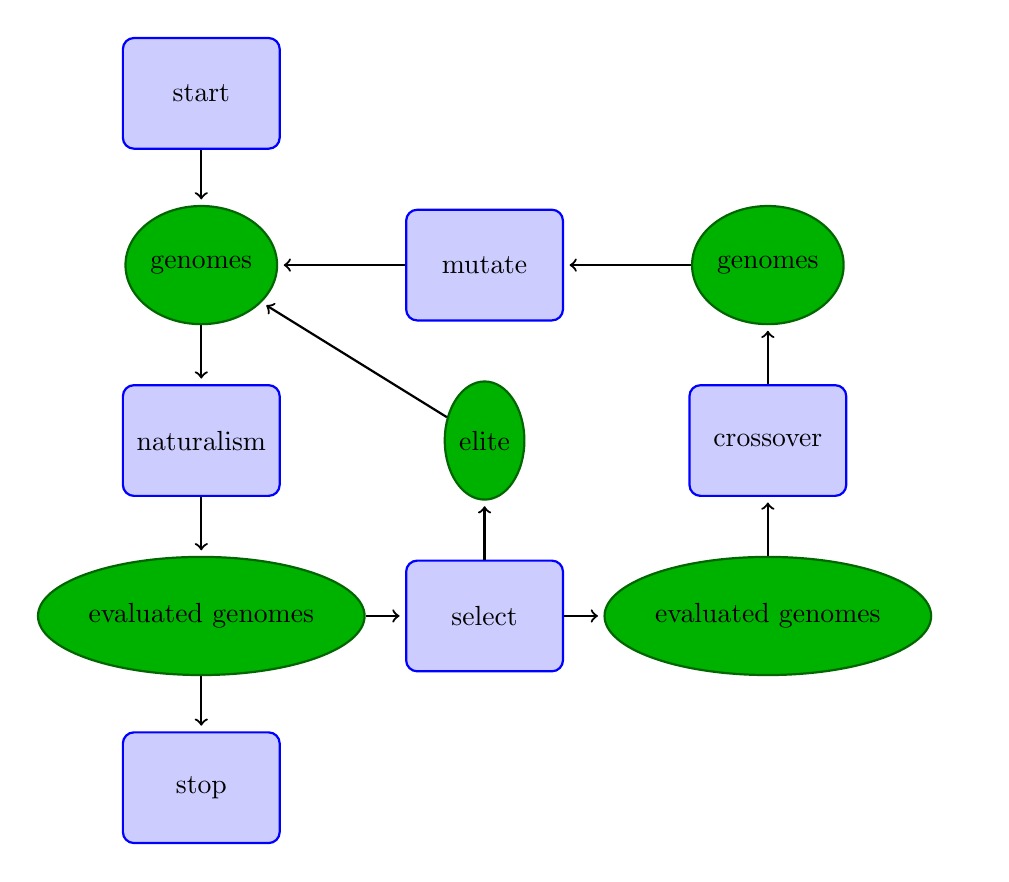
\begin{tikzpicture}
	[auto,
		decision/.style	={diamond, draw=blue, thick, fill=blue!20,
									text width=4.5em,align=flush center,
									inner sep=1pt},
		block/.style		={rectangle, rounded corners, draw=blue, thick, fill=blue!20,
									text width=5em,align=center,
									minimum height=4em},
		line/.style		 	={draw, thick, ->,shorten >=2pt},
		cloud/.style		={ellipse, rounded corners, draw=green!40!black, thick,fill=green!70!black,
									minimum height=1.5cm,inner sep=1pt}
	]
\matrix [column sep=5mm,row sep=7mm]
	{
		% row 1
			\node [block] (start) {start}; & 
		\\
		% row 2
			\node [cloud] (genomes 1)						{genomes}; &
			\node [block] (mutate)							{mutate}; &
			\node [cloud] (genomes 2)						{genomes}; &
		 \\
		% row 3
			\node [block] (naturalism)						{naturalism}; &
			\node [cloud] (elite)								{elite}; & 
			\node [block] (crossover)						{crossover}; &
			%\node [cloud, dashed] (random)							{random}; &
		\\
		% row 4
			\node [cloud] (evaluated genomes 1)	{evaluated genomes}; & 
			\node [block] (select)								{select}; & 
			\node [cloud] (evaluated genomes 2)	{evaluated genomes}; &
		\\
		% row 5
			\node [block] (stop)								{stop}; &
		\\
	};
\begin{scope}[every path/.style=line]

	\path					(start)				-- (genomes 1);

	\path					(mutate) 		-- (genomes 1);
	\path					(genomes 2) 		-- (mutate);

	\path					(genomes 1) 		-- (naturalism);
	\path					(elite) 		-- (genomes 1);
	\path					(crossover) 		-- (genomes 2);

	%\path	[dashed]	(random)-- (crossover);

	\path					(naturalism)	-- (evaluated genomes 1);
	\path					(select)	-- (elite);
	\path					(evaluated genomes 2)-- (crossover);

	\path					(evaluated genomes 1) --(select);
	\path					(select)	-- (evaluated genomes 2);

	\path					(evaluated genomes 1) --(stop);
	
%	\path					(update)		|- (identify);
%	\path					(decide)		-| node [near start] {yes} (update);
%	\path					(decide)		-- node [midway] {no} (stop);
%	\path [dashed]	(expert)		-- (init);
%	\path [dashed]	(system)		-- (init);
%	\path [dashed] 	(system)		|- (evaluate);
\end{scope}
\end{tikzpicture}

